\section{Background on Modulo Unrolling}\label{sec:modulo_unrolling}

Modulo unrolling \cite{barua1999maps} is a static disambiguation method used in tiled architectures that is applicable to loops with affine array accesses. An affine function of a set of variables is defined as a linear combination of those variables. An affine array access is any array access where each dimension of the array is accessed by an affine function of the loop induction variables. For example, for loop index variables $i$ and $j$ and array $A$, $A[i+2j+3][2j]$ is an affine access, but $A[ij+4][j^2]$ and $A[2i^2+1][ij]$ are not. 

Modulo unrolling works by unrolling the loop by a factor equal to the number of memory banks on the architecture. If the arrays accessed within the loop are distributed using low-order interleaving (a Cyclic distribution), then after unrolling, each array access will be \textit{statically disambiguated}, or guaranteed to reside on a single bank for all iterations of the loop. This is achieved with a modest increase of the code size. 

To understand modulo unrolling, refer to Figure~\ref{modulo_unrolling}. In Figure~\ref{modulo_unrolling}a there is a code fragment consisting of a sequential \textbf{for} loop with a single array access $A[i]$. The array $A$ is distributed over four memory banks using a Cyclic distribution. As is, the array $A$ is not statically disambiguated because accesses of $A[i]$ go to different memory banks on different iterations of the loop. The array access $A[i]$ has bank access patterns 0, 1, 2, 3, 0, 1, 2, 3, ... in successive loop iterations. 

A naive approach to achieving static disambiguation is to fully unroll the loop, as shown in Figure~\ref{modulo_unrolling}b. Here, the original loop is unrolled by a factor of 100. Because each array access is independent of the loop induction variable $i$, static disambiguation is achieved trivially. Each array access resides on a single memory bank. However, fully unrolling the loop is not an ideal solution to achieving static disambiguation because of the large increase in code size. This increase in code size is bounded by the unroll factor, which may be extremely large for loops iterating over large arrays. Fully unrolling the loop may not even be possible for a loop bound that is unknown at compile time. 

A more practical approach to achieving static disambiguation without a dramatic increase in code size is to unroll the loop by a factor equal to the number of banks on the architecture. This is shown in Figure~\ref{modulo_unrolling}c and is known as modulo unrolling. Since we have 4 memory banks in this example, we unroll the loop by a factor of 4. Now every array reference in the loop maps to a single memory bank on all iterations of the loop. Specifically, $A[i]$ refers to bank 0, $A[i+1]$ refers to bank 1, $A[i+2]$ refers to bank 2, and $A[i+3]$ refers to bank 3. The work in \cite{barua1999maps} shows that an unroll factor providing this property always exists not only for the code in Figure \ref{modulo_unrolling}, but for the general case of any affine function in a loop.  The unroll factor may not always equal the number of banks, but a suitable unroll factor can always be computed.

Modulo unrolling, as used in \cite{barua1999maps} provides static disambiguation and memory parallelism for tiled architectures. That is, after unrolling, each array access can be done in parallel because array accesses map to a different memory banks. 

\begin{figure}
\begin{center}
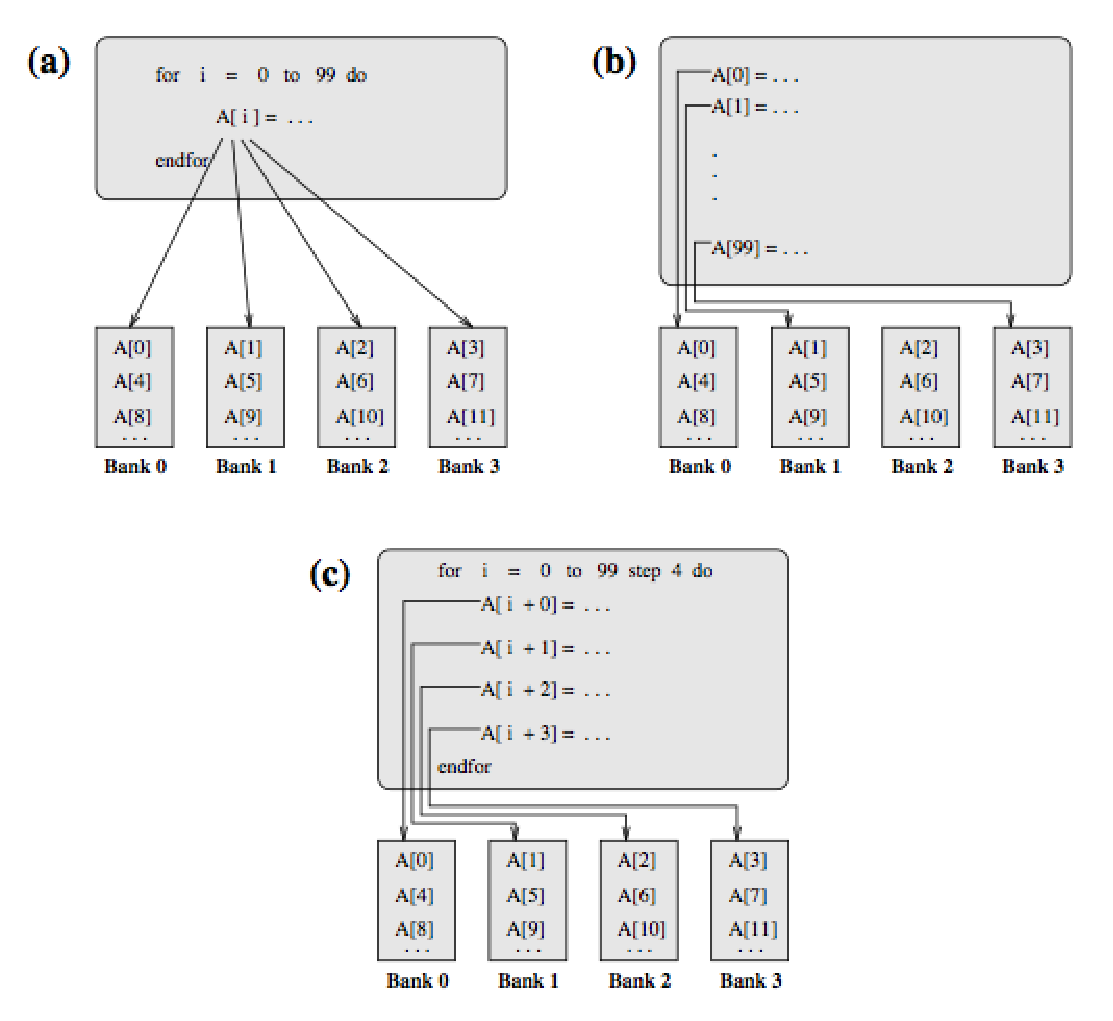
\includegraphics[scale=0.45]{./Figures/modulo_unrolling.eps}
\caption{Modulo unrolling example. (a) Original sequential for loop. Array $A$ is distributed using a Cyclic distribution. Each array access maps to a different memory bank on successive loop iterations. (b) Fully unrolled loop. Trivially, each array access maps to a single memory bank because each access only occurs once. This loop dramatically increases the code size for loops traversing through large data sets. (c) Loop transformed using modulo unrolling. The loop is unrolled by a factor equal to the number of memory banks on the architecture. Now each array access is guaranteed to map to a single memory bank for all loop iterations and code size increases only by the loop unroll factor.}
\label{modulo_unrolling}
\end{center}
\end{figure}